\documentclass[UTF8,a4paper,11pt]{ctexart}
\usepackage[margin=2.1cm]{geometry}
\usepackage{amsmath,amssymb}
\usepackage{booktabs}
\usepackage{graphicx}
\usepackage{hyperref}
\usepackage{caption}
\hypersetup{colorlinks=true,linkcolor=blue,urlcolor=blue}
\setlength{\parindent}{2em}
\setlength{\parskip}{0.25em}
\newcommand{\NL}{N_{\mathrm L}}
\newcommand{\NF}{N_{\mathrm F}}

\title{密集跟随式 LEO 网络的资源一致 SINR 结果分析}
\author{Comprehensive numerical analysis}
\date{\today}

\begin{document}
\maketitle

\section{分析原则}

本文结果使用固定总地面带宽的集群内正交资源模型作为主模型。每个 cluster 的 leader
和 followers 分享地面带宽，不再给每个服务分支同时分配完整带宽。不同 clusters 复用
同一资源块图样。复用因子为 $K_{\rm reuse}$ 时，每个 cluster 只使用总频谱的
$1/K_{\rm reuse}$，因此所有速率均包含复用带宽代价。结果同时报告接入覆盖、端到端
relay coverage、cluster rate 与 network throughput proxy，以避免只根据单一平均指标给出结论。

默认协调场景采用复用因子 $K_{\rm reuse}=3$、活动概率 $p_{\rm act}=0.5$ 和干扰耦合
增益 $G_{\rm I}=-20$ dB。该场景不是宣称固定的工程参数，而是用于展示频率复用、调度
与波束隔离共同作用后的可实现设计区间。这里 $p_{\rm act}$ 表示典型资源块已调度条件下
的同频重叠概率，不是整个 cluster 的全局 duty cycle。Fig.S5 对这些参数进行了显式
敏感性分析。

\section{资源模型决定干扰结论}

\begin{figure}[htbp]
\centering
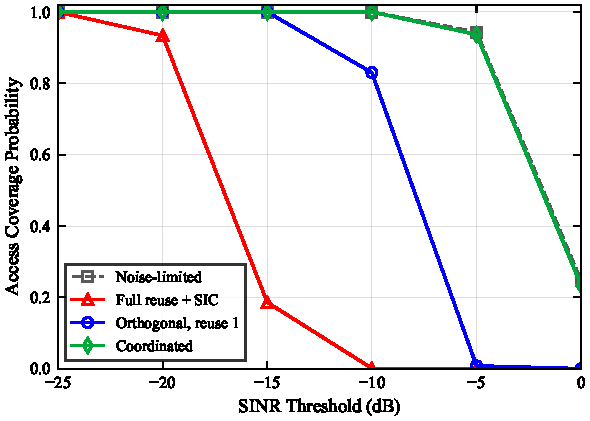
\includegraphics[width=0.78\linewidth]{../figures/sinr/figS1_resource_model_coverage.pdf}
\caption{不同资源模型下的接入覆盖概率。}
\label{fig:s1}
\end{figure}

图 \ref{fig:s1} 表明，网络是否“干扰受限”不能脱离资源模型讨论。在
$\NL=1000,\NF=10$ 时，噪声受限场景在 $-5$ dB 的接入覆盖约为 $0.943$；协调场景
约为 $0.937$，说明复用、稀疏活动与旁瓣隔离可以使密集网络接近噪声受限性能。相比之下，
正交资源但集群间 reuse-1、且干扰耦合为 $0$ dB 时，$-5$ dB 接入覆盖仅约 $0.008$。

Full reuse + SIC 是极端基准：所有外部 leader/follower 同频，但服务 cluster 内采用理想
SIC。在 $-15$ dB 时其接入覆盖约为 $0.176$，在 $-10$ dB 的 $1000$ 次试验中未观察到
成功事件。Wilson 95\% 区间上界约为 $0.0038$，因此这里应解释为“概率很低”，而不是
真实概率严格为零。

\section{接入覆盖不等于端到端覆盖}

\begin{figure}[htbp]
\centering
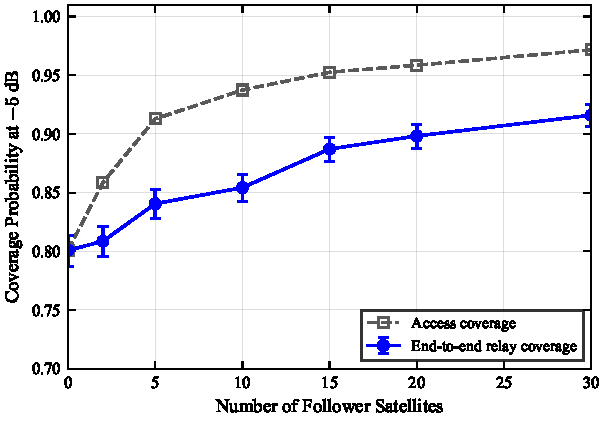
\includegraphics[width=0.78\linewidth]{../figures/sinr/figS2_access_vs_e2e.pdf}
\caption{协调场景中接入覆盖与端到端 relay coverage 的差异。}
\label{fig:s2}
\end{figure}

图 \ref{fig:s2} 使用 $-5$ dB 地面门限和 $-5$ dB leader--follower 门限。随着
$\NF$ 从 $0$ 增加到 $30$，接入覆盖从约 $0.801$ 提升到 $0.972$；端到端覆盖从约
$0.801$ 提升到 $0.916$。两者之间的差距来自星间回传瓶颈：一个 follower 即使具有
足够强的地面 SINR，也必须先从 leader 成功获得数据。

因此，以地面最大 SINR 定义的 coverage 会高估译码转发系统的实际可靠性。后续网络设计
应优先使用端到端 coverage，接入 coverage 只作为诊断指标。

\section{固定总带宽下的 follower 数量权衡}

\begin{figure}[htbp]
\centering
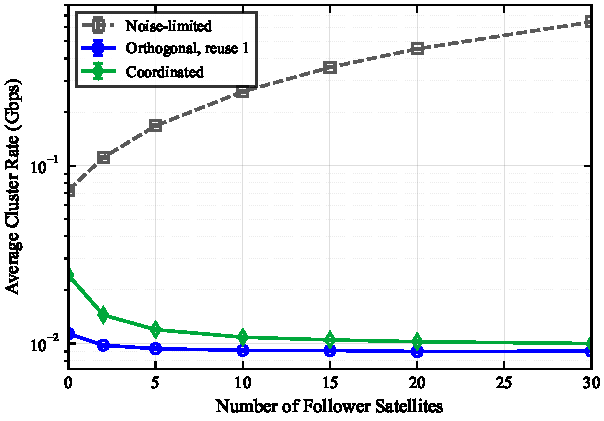
\includegraphics[width=0.78\linewidth]{../figures/sinr/figS3_rate_resource_models.pdf}
\caption{不同资源模型下平均 cluster rate 随 follower 数量的变化。}
\label{fig:s3}
\end{figure}

图 \ref{fig:s3} 揭示了固定总资源模型与原噪声受限逐分支全带宽模型之间的根本差异。
在噪声受限逐分支全带宽基准中，$\NF=0$ 到 $30$ 时平均速率从约 $0.0726$ Gbps
增至 $0.6435$ Gbps。该趋势代表增加并行资源后的上界，而不是固定总带宽下的公平比较。

在协调、固定总带宽且 $K_{\rm reuse}=3$ 的场景中，$\NF=0$ 时平均 cluster rate
约为 $0.0242$ Gbps；$\NF=10$ 时降至约 $0.0108$ Gbps；$\NF=30$ 时约为
$0.0100$ Gbps。与此同时，
端到端覆盖从约 $0.795$ 提升到 $0.915$。因此 followers 的主要价值是可靠性和空间
分集，而不是在固定资源下无条件增加总速率。

在正交 reuse-1 且无旁瓣隔离的场景中，速率约为 $0.009$--$0.011$ Gbps，端到端覆盖
接近零。这个结果说明：若不进行干扰管理，单纯增加 followers 无法修复密集同频网络。

\section{网络密度与聚合吞吐}

\begin{figure}[htbp]
\centering
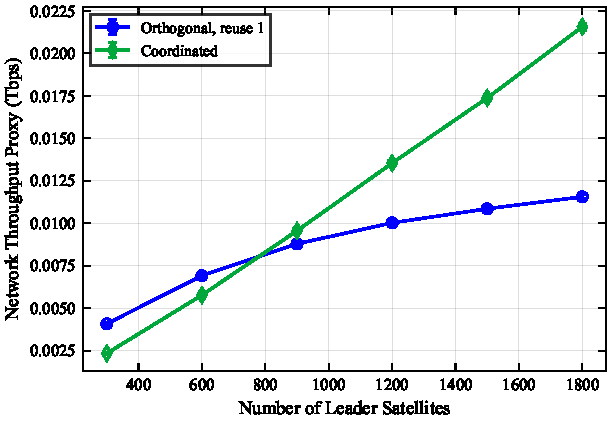
\includegraphics[width=0.78\linewidth]{../figures/sinr/figS4_network_throughput.pdf}
\caption{$\NF=10$ 时网络聚合吞吐代理随 leader 数量变化。}
\label{fig:s4}
\end{figure}

图 \ref{fig:s4} 中，reuse-1 场景的 network throughput proxy 随 $\NL$ 增加缓慢趋于饱和：
$\NL=300$ 时约为 $0.0041$ Tbps，$\NL=1800$ 时约为 $0.0116$ Tbps；与此同时，
端到端覆盖从约 $0.150$ 下降到在有限样本中未观察到成功。仅看聚合吞吐会掩盖严重的
可靠性损失。

协调场景中，$\NL=300$ 到 $1800$ 时 network throughput proxy 从约 $0.00234$ Tbps 增至
$0.0216$ Tbps，端到端覆盖也从约 $0.614$ 提升到 $0.924$。覆盖随 $\NL$ 提升的原因是
最近服务 leader 距离缩短，而协调参数将新增干扰限制在较低水平。该结果说明网络密度
本身不是问题，关键是新增空间复用收益是否伴随相应的干扰隔离。这里的 proxy 假定每个
cluster 有一个已调度代表用户；因为未定义用户点过程与业务负载，它不能直接解释为真实
运营网络的总吞吐。CSV 同时给出按地球表面积和总带宽归一化的 spherical spectral
efficiency proxy。

\section{协调参数敏感性}

\begin{figure}[htbp]
\centering
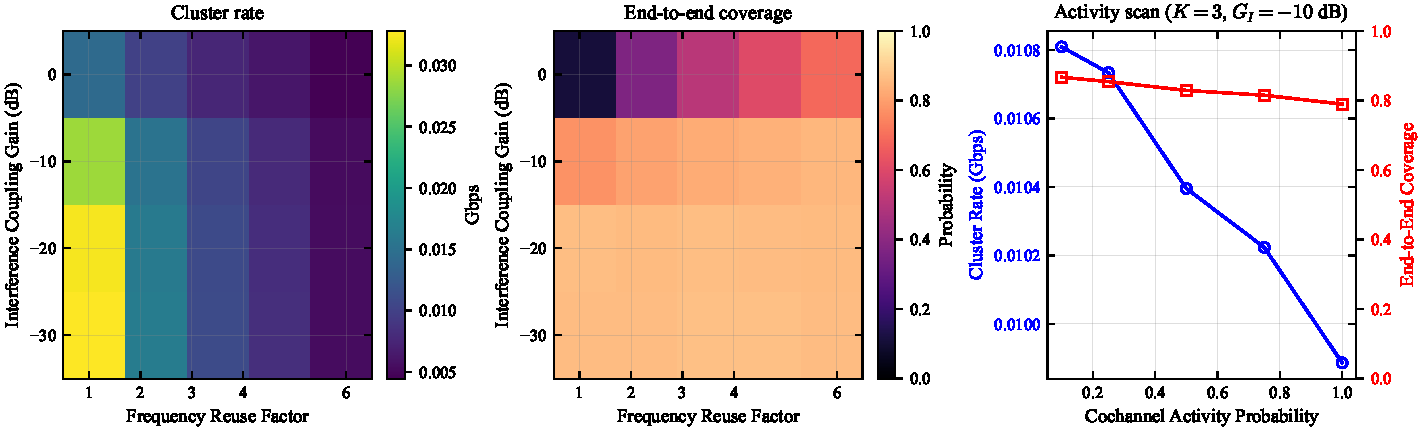
\includegraphics[width=0.98\linewidth]{../figures/sinr/figS5_coordination_sensitivity.pdf}
\caption{复用因子和干扰耦合增益对 cluster rate 与端到端覆盖的联合影响。}
\label{fig:s5}
\end{figure}

图 \ref{fig:s5} 的两个热图固定同频活动概率为 $0.5$。当干扰耦合接近 $0$ dB 时，
提高复用因子可把端到端覆盖从约 $0.108$ 提升到 $0.687$，但由于每集群带宽按
$1/K_{\rm reuse}$ 缩小，平均速率仍从约 $0.0143$ Gbps 降至 $0.00446$ Gbps。
当耦合低于 $-20$ dB 时，覆盖已接近饱和，继续提高复用因子主要产生频谱损失。

右侧活动概率扫描固定 $K_{\rm reuse}=3,G_{\rm I}=-10$ dB。同频活动概率从 $0.1$
增至 $1$ 时，平均速率从约 $0.01081$ Gbps 降至 $0.00989$ Gbps，端到端覆盖从
$0.867$ 降至 $0.790$。因此调度稀疏化能够改善可靠性，但其系统代价需要结合业务负载
与时延另行评估。该图避免了只选择单一协调参数后得出过度一般化结论。

工程上，复用因子会减少频谱复用效率，而较低干扰耦合通常需要更窄波束、更精确指向或
更严格调度。因此，最优设计应联合考虑频谱、天线和调度成本，而不是只追求最低 INR。

\section{半解析模型验证}

\begin{figure}[htbp]
\centering
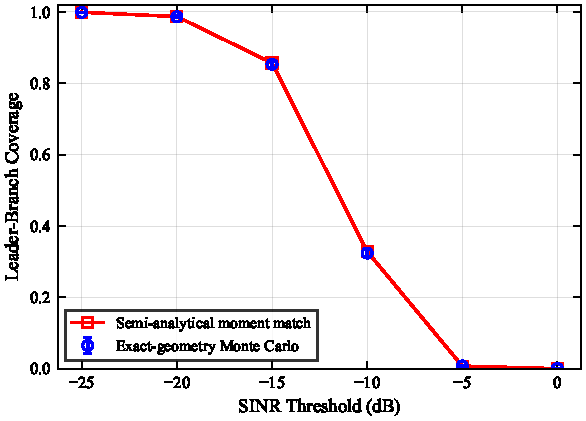
\includegraphics[width=0.78\linewidth]{../figures/sinr/figS6_semi_analytical_validation.pdf}
\caption{条件矩匹配半解析 leader coverage 与完整几何 Monte Carlo 对比。}
\label{fig:s6}
\end{figure}

图 \ref{fig:s6} 显示半解析曲线与完整几何 Monte Carlo 高度一致。在扫描门限内，最大
绝对误差约为 $0.0048$；例如 $-10$ dB 时半解析值为 $0.3289$，Monte Carlo 为
$0.3241$。独立 validation gate 使用不同随机种子和参数，得到的最大绝对误差约为
$0.0157$，仍低于预设 $0.04$ 阈值。

此外，moment-matched cluster-rate 与共享外部集群几何的完整 Monte Carlo 相对误差
约为 $1.56\%$，端到端覆盖绝对误差约为 $0.0028$。这些结果支持使用矩匹配方法进行
大规模参数扫描，同时保留完整几何 Monte Carlo 作为最终验证。

\section{可见边界修正}

\begin{figure}[htbp]
\centering
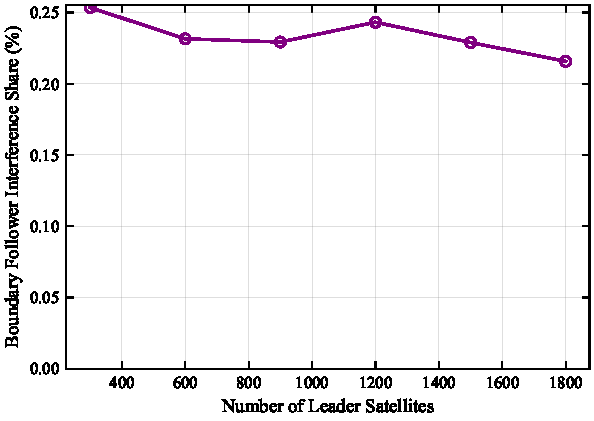
\includegraphics[width=0.78\linewidth]{../figures/sinr/figS7_boundary_correction.pdf}
\caption{parent leader 不可见但 follower 可见所贡献的平均 follower 干扰比例。}
\label{fig:s7}
\end{figure}

图 \ref{fig:s7} 量化了可见边界修正。在默认 $1^\circ$ follower 球冠下，旧的
“parent leader 不可见则整个 cluster 不干扰”处理会漏掉约 $0.22\%$--$0.25\%$ 的
平均 follower 干扰。该比例较小，因此不会改变默认参数下的总体趋势；但它严格非零，
并且在更大 cluster radius、不同波束或更低轨道场景中可能增大。最终代码已经按 follower
自身可见性判断干扰，不再依赖 parent leader 的可见性。

\section{速率--可靠性前沿}

\begin{figure}[htbp]
\centering
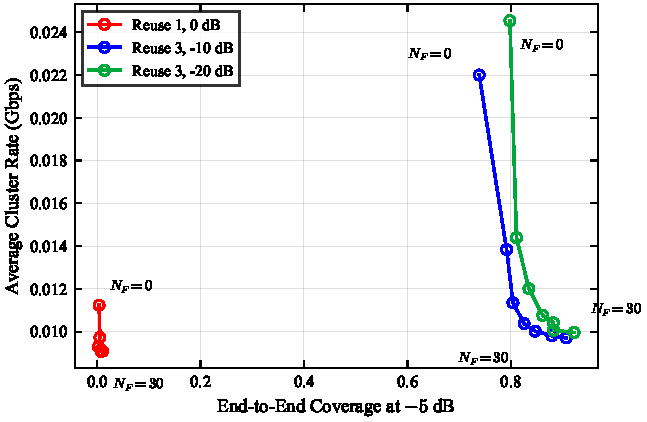
\includegraphics[width=0.78\linewidth]{../figures/sinr/figS8_rate_reliability_frontier.pdf}
\caption{不同协调强度下，改变 follower 数量形成的速率--可靠性前沿。}
\label{fig:s8}
\end{figure}

图 \ref{fig:s8} 将 follower 数量选择转化为多目标设计问题。reuse-1、$0$ dB 耦合场景
同时具有低速率和低可靠性，不构成有吸引力的设计区域。复用因子 $3$ 且耦合为
$-10$ dB 或 $-20$ dB 时，增加 followers 可将端到端覆盖提升到约 $0.907$ 或
$0.922$，但平均速率下降到约 $0.0097$--$0.0100$ Gbps。

因此不存在脱离业务目标的唯一“最佳 follower 数量”。吞吐优先业务倾向较少 followers；
高可靠业务可以增加 followers，并接受带宽分割造成的速率损失。实际选择应在端到端
coverage 约束下最大化 cluster rate，或在最低速率约束下最大化可靠性。

\section{最终结论}

\begin{enumerate}
  \item 密集 LEO 网络的干扰结论高度依赖资源模型。极端全同频模型适合作为下界，但不能
  直接代表具有复用、调度和波束隔离的实际系统。
  \item 在固定总地面带宽下，增加 followers 的主要收益是提高接入与端到端可靠性；其
  代价是每个资源块带宽下降，平均 cluster rate 通常降低。
  \item 接入 coverage 会忽略 leader--follower 回传瓶颈，必须使用端到端 coverage
  评价译码转发系统。
  \item 复用因子、活动概率和干扰耦合增益共同决定网络能否从干扰受限转向近噪声受限；
  频率复用同时付出 $1/K_{\rm reuse}$ 带宽代价，必须联合比较速率与覆盖。
  \item 条件矩匹配半解析模型与完整几何 Monte Carlo 在当前参数域内一致，可用于快速
  网络设计扫描；关键结论均由完整几何或独立 validation gate 复核。
\end{enumerate}

\section{结论边界}

上述结果建立在球面 BPP、统一干扰耦合增益、快照几何、均匀带宽划分以及方向性/正交
ISL 的假设上。它们能够回答“密集网络中增加 followers 与干扰管理之间的基本权衡”，
但不能直接替代真实星座的波束图、轨道动态、切换、业务到达与调度优化。特别是默认
$G_{\rm I}=-20$ dB 协调场景是参数化设计点，不是未经实测即可保证的工程值。

\end{document}
